\documentclass[12pt]{article}
\usepackage{geometry}                % See geometry.pdf to learn the layout options. There are lots.
\geometry{letterpaper}                   % ... or a4paper or a5paper or ...
%\geometry{landscape}                % Activate for for rotated page geometry
%\usepackage[parfill]{parskip}    % Activate to begin paragraphs with an empty line rather than an indent
\usepackage{graphicx}
\usepackage{amssymb}
\usepackage{amsmath}
\usepackage{epstopdf}
\usepackage{wrapfig}
\usepackage{natbib}
%\usepackage[square,comma,numbers,sort]{natbib}
\usepackage[pdftex, plainpages=false, colorlinks=true, linkcolor=blue, citecolor=blue, bookmarks=false]{hyperref}
\usepackage{setspace}
\usepackage{multicol}
\usepackage{sectsty}
\usepackage{url}
\usepackage{lipsum}
\usepackage{times}
\usepackage[tiny,compact]{titlesec}
\usepackage{fancyhdr}
\usepackage{deluxetable}
\usepackage[font=footnotesize,labelfont=bf]{caption}
\usepackage{verbatim}
\usepackage{acronym}

\setlength{\textwidth}{6.5in}
\setlength{\oddsidemargin}{0.0cm}
\setlength{\evensidemargin}{0.0cm}
\setlength{\topmargin}{-0.5in}
\setlength{\headheight}{0.2in}
\setlength{\headsep}{0.2in}
\setlength{\textheight}{9.in}
%\setlength{\footskip}{-0.2in}
%\setlength{\voffset}{0.0in}

\sectionfont{\normalsize}
\subsectionfont{\normalsize}
\subsubsectionfont{\normalsize}
\singlespacing

\input ../macros.tex
\input ../journal_abbr.tex

\pagestyle{fancy}
\fancyhf{}
\lhead{\fancyplain{}{\doctitle}}
\rhead{\fancyplain{}{S.M. Couch}}
\rfoot{\fancyplain{}{\thepage}}

\bibliographystyle{aasjournal}
%\bibliographystyle{hapj}
%\bibliographystyle{physrev}



%\titlespacing*{\section}{0in}{0.2in}{0in}
%\titlespacing*{\subsection}{0in}{0.1in}{0in}
\titleformat*{\subsection}{\itshape}
%\titlespacing*{\subsubsection}{0in}{0.in}{0in}
\titleformat*{\subsubsection}{\itshape}
\setlength{\abovecaptionskip}{3pt}

\begin{document}

\begin{center}
  {\bf Year 2 - CY2019 Allocation Renewal} \vspace{-0.1in}
\end{center}

\section*{Achievements in Year 1}

\section{Progress on Year 1 Milestones}

\subsection{3D simulations of magnetorotational core-collapse supernovae}

One of the key objectives for Year 1 of our INCITE project was to execute a parameter study of magnetorotational core-collapse supernova (CCSN) simulations using high-fidelity neutrino transport and magnetohydrodynamics (MHD) as implemented in our \sparkmone application, built in the \flash simulation framework \citep{Fryxell:2000, Dubey:2009}.
\sparkmone utilizes the new \spark high-order MHD solver \citep{couch:2017}, the M1 two-moment explicit neutrino transport method \citep{Shibata:2011a, oconnor:2015, oconnor:2018}, an accurate and efficient multipole gravity solver \citep{couch:2013c} including the general relativistic monopole correction \citep{Marek:2006}, an approximate 21-isotope nuclear network for accurately tracking the composition at low densities \citep{couch:2015a}, and the \flash framework for adaptive mesh refinement (AMR), I/O, and runtime management.
The methods and physics included in \sparkmone make it one of the most high-fidelity and high-performance CCSN simulation tools in the world.

\begin{figure*}[b!]
  \begin{tabular}{ccc}
    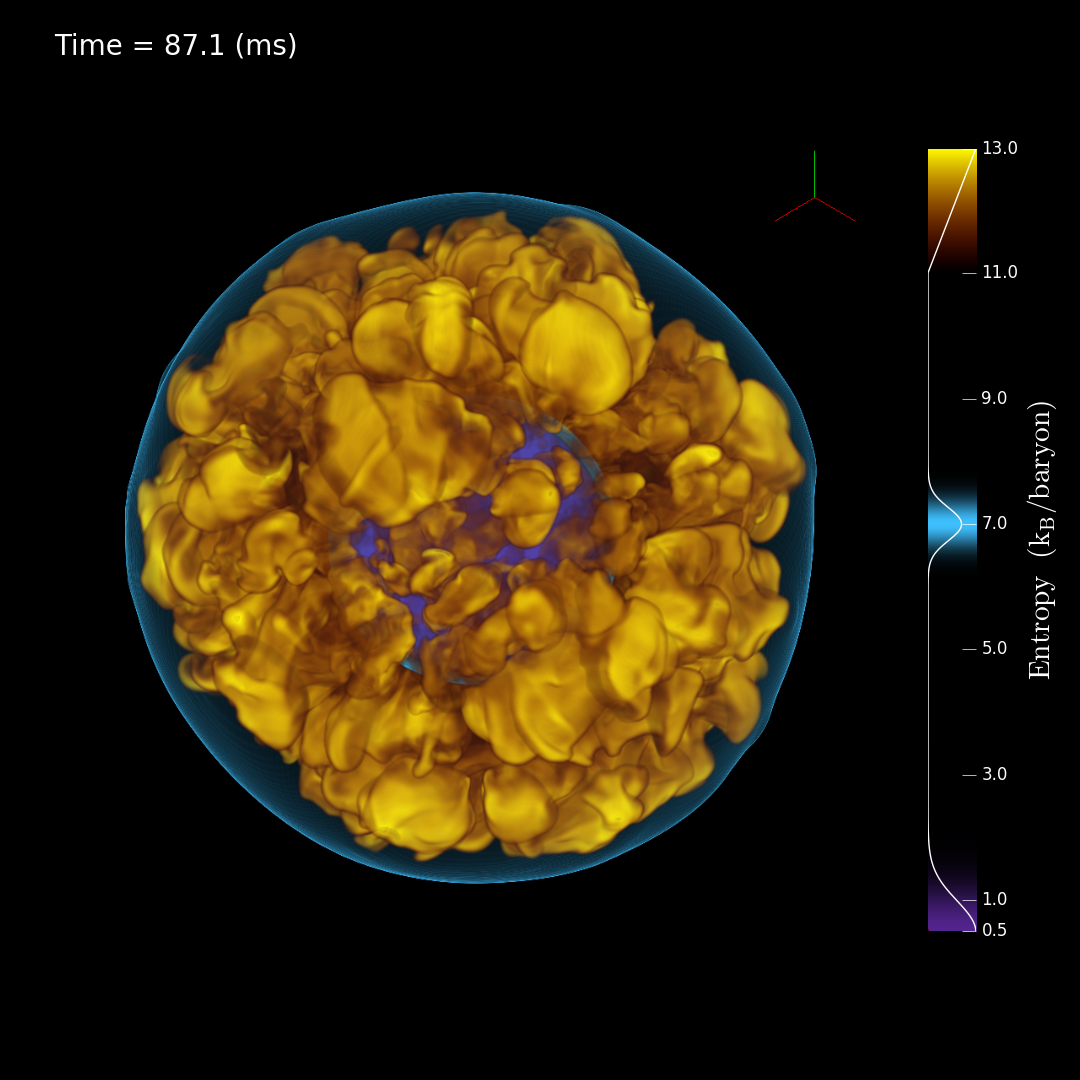
\includegraphics[width=2in]{fig_vr_m15u_3d_mag_annotated_0677.png} &
    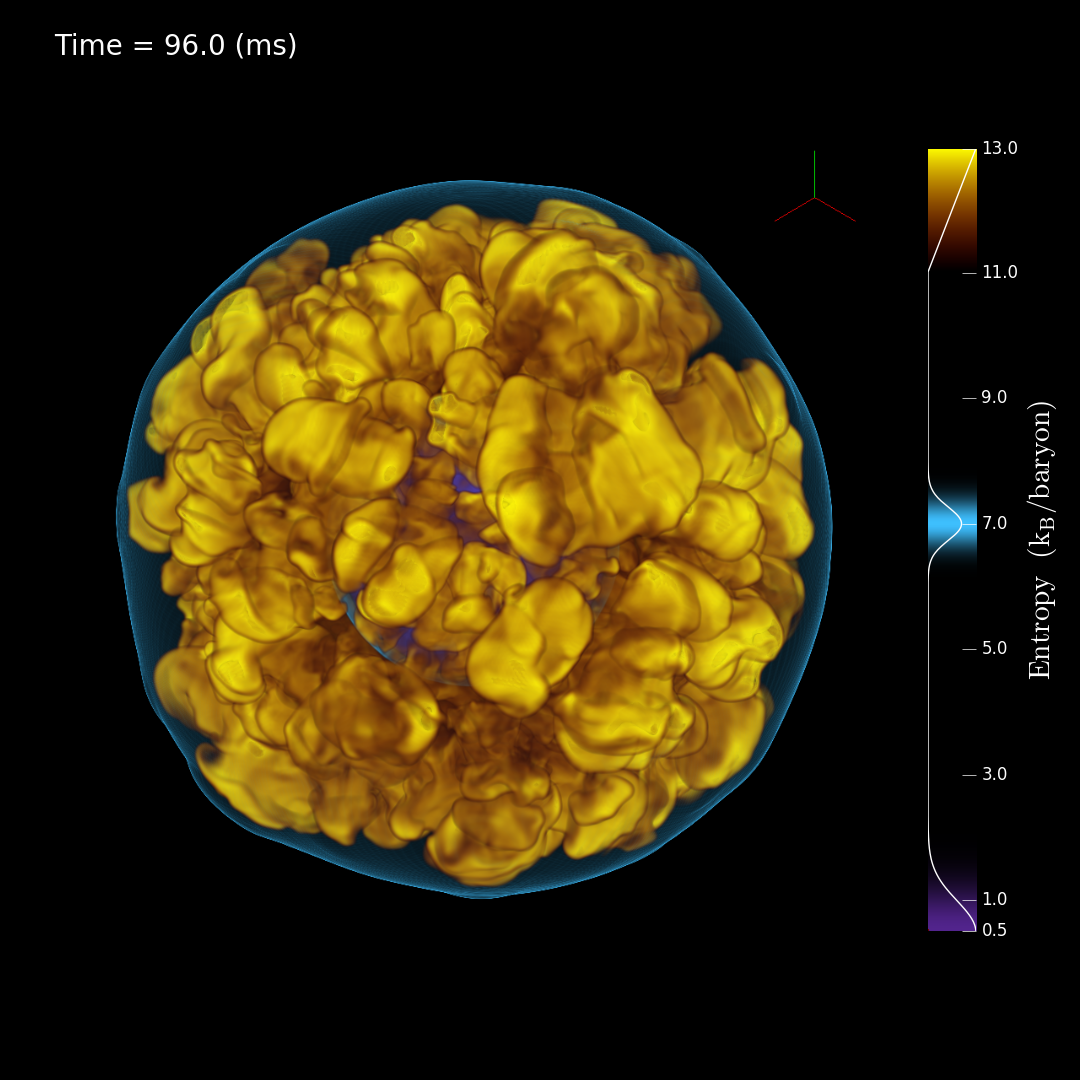
\includegraphics[width=2in]{fig_vr_m15u_3d_mag_rot_annotated_0695.png} &
    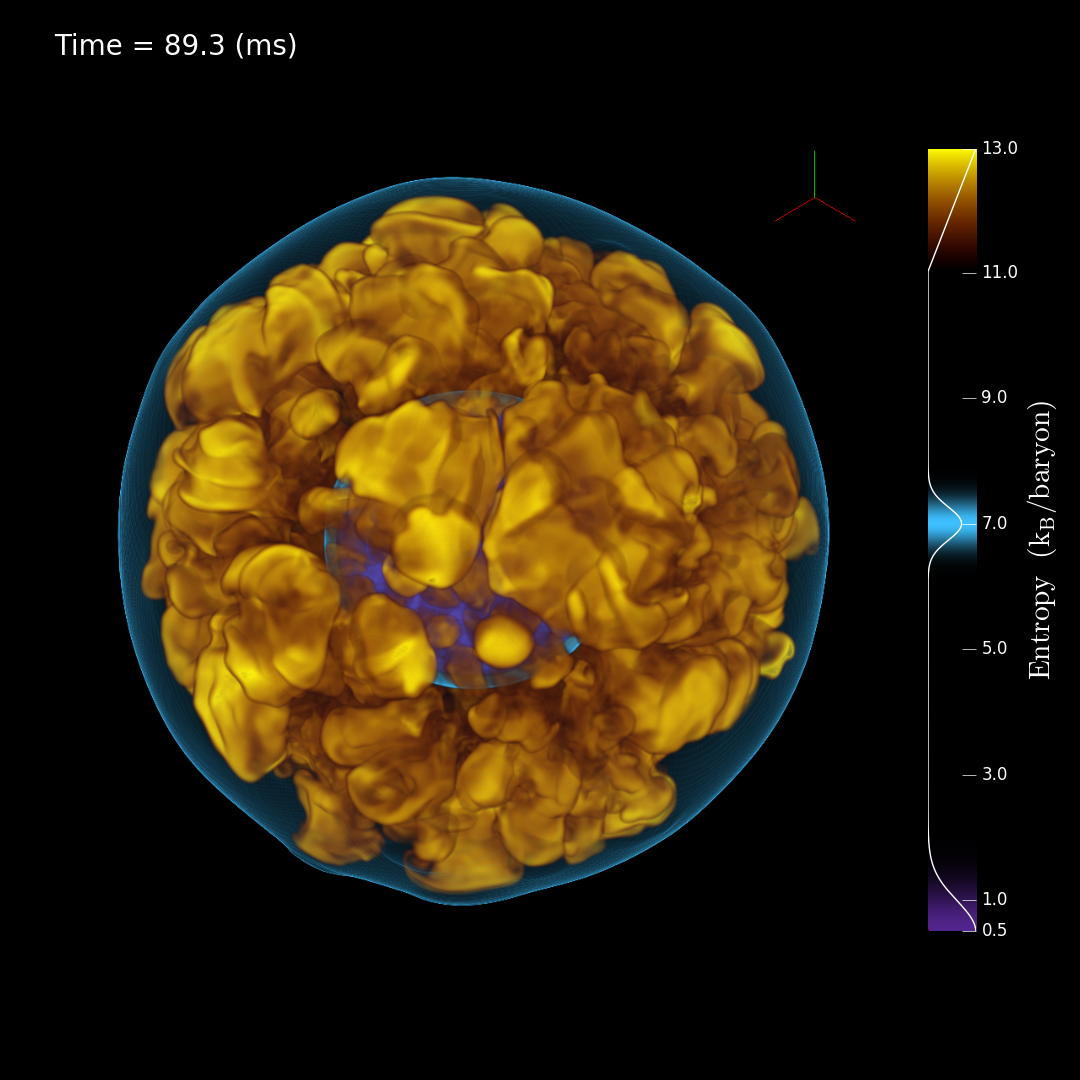
\includegraphics[width=2in]{./fig_vr_m15u_3d_rot2_annotated_0696.png}    
  \end{tabular}
  \caption{Volume renderings of entropy from three of the 3D magnetorotational CCSN simulations that we are currently running on \mira as part of this INCITE project. Shown are cases with magnetic fields (left), magnetic fields and rotation (middle), and no magnetic fields but fast rotation (right). All of these simulations are currently at around 100 ms post-bounce and are on-going.} 
  \label{f.m15u}
\end{figure*}

The \spark MHD solver \citep{couch:2018} implements the cell-centered method of generalized Lagrangian multipliers \citep[GLM;][]{Dedner:2002, Mignone:2010} to control the growth of the divergence of the magnetic field. 
The GLM-MHD scheme employs hyperbolic advection and parabolic damping of divergence errors in order to avoid expensive elliptic divergence cleaning \citep[e.g.,][]{Jiang:1999} or complicated staggered-mesh constrained transport \citep[e.g.,][]{Gardiner:2005, Lee:2009a, Lee:2013}.
\spark implements the GLM-MHD scheme via a finite-volume approach using high-order primitive reconstruction, multiple Riemann solvers for flux calculation, and method-of-lines time integration using multi-stage strong stability preserving (SSP) low-storage Runge-Kutta (RK) integrators of second- and third-order \citep[e.g.,][]{Gottlieb:1998}.
For realistic, non-Gamma-law equations of state, \spark avoids the approach of \citet{Colella:1985} used in other \flash solvers and adopts the volumetric internal energy, $\rho e$, as an auxiliary thermodynamic primitive variable instead, as in \citet{Almgren:2010}.
We have found this approach to be generally more robust but either method should be technically equivalent \citep[e.g.,][]{Zingale:2015}.
For our CCSN application, we use fifth-order WENO reconstruction \citep{Borges:2008}, second-order time integration, and the HLLD approximate Riemann solver which includes MHD waves \citep{Miyoshi:2005}.



Neutrino transport in \sparkmone is carried out using the M1 two-moment explicit approach described in \citet{oconnor:2015, oconnor:2018, oconnor:2018b}. 
The M1 scheme solves the first two angular moments of the Boltzmann equation for neutrinos and utilizes an analytic closure for the higher-order moments.
The neutrino fluxes, both in real space and in energy space, are computed explicitly as a hyperbolic system resulting in favorable performance and scaling properties (at the cost of time step sizes limited by the speed of light) while the matter-radiation source terms are computed implicitly.
This implicit solve is completely local and requires solving only a 4x4 matrix.
Our M1 solver is fully velocity-dependent, except in the calculation of the explicit flux terms, which is done to $\mathcal{O}(v/c)$.
We currently do not include inelastic neutrino scattering in the multidimensional version of our transport solver although inelastic neutrino electron scattering is included in the 1D implementation in GR1D \citep{oconnor:2015}.
We plan to implement and include inelastic scattering in our 3D simulations in Years 2 and 3 of this project.

The two-moment M1 approach is inherently more accurate than zeroth-moment only approaches such as flux-limited diffusion \citep[e.g.,][]{bruenn:2013, Dolence:2015, Lentz:2015}. 
M1 does not require a flux-limiter-based closure for the radiation fluxes as they are solved for directly.
Furthermore, the analytic closure we currently use for the moments beyond the first is simple and straightforward yet shows encouraging agreement with 1D Boltzmann and Monte Carlo neutrino transport calculations \citep{oconnor:2015, Murchikova:2017}.
As compared with flux-limited diffusion, M1 does not suffer from the inability to capture ``shadows'' inherent to FLD schemes.
A known limitation of M1 is cases in which distinct beams of radiation intersect, causing radiation ``shocks.''
The M1 solution in such cases becomes highly diffuse at the intersection.
This is a problem in, e.g., radiation hydrodynamic calculations of accretion disks.
For CCSNe, however, the radiation field is highly forward peaked and cases in which distinct beams of radiation might cross are essentially non-existent.
Hence, M1 is {\it ideally} suited for the CCSN problem due to its accuracy (for the specific problem) and efficiency.
In addition, the severe limitation of time steps determined by the speed of light is not so drastic in CCSNe since the explicit time step is already just a factor of a few larger than this thanks to the enormous sound speeds in the proto-neutron star (PNS).
Another significant advantage of M1 is that it is a fully multidimensional transport scheme, i.e., the solution at a given grid point is dependent on the fluxes from every direction around that point.
This is distinct from the often-adopted ``ray-by-ray'' approximation \citep[e.g.,][]{bruenn:2013, bruenn:2016, muller:2012a, Hanke:2013, Melson:2015, Lentz:2015} in which the transport problem is solved only along discrete radial rays.
The advantages of M1 for neutrino transport in CCSNe have not gone unnoticed and a number of groups are now exploring or adopting this approach \citep{Just:2015, Kuroda:2016, Skinner:2016, Roberts:2016}.


In our \flash CCSN application we have assumed that the composition of the matter throughout the entire computational domain is determined by nuclear statistical equilibrium (NSE).
This common approximation \citep[e.g.,][]{Burrows:2007, Ott:2008, Dolence:2015, Skinner:2016, Roberts:2016, Kuroda:2016} is appropriate at high densities and temperatures where the nuclear reaction rates are sufficiently fast to establish equilibrium essentially instantly but becomes increasingly incorrect at low densities such as those in the silicon and oxygen shells surrounding the collapsing iron core.
Critically, correctly predicting the explosion energy or nucleosynthetic products such as radioactive nickel can be severely impacted by the inappropriate assumption of NSE \citep{bruenn:2016}.
\citet{bruenn:2016} advocate the use of an approximate nuclear network in regions that are not in NSE, while other groups \citep[e.g.,][]{muller:2012a, Melson:2015} use a ``flashing'' approach rather than a full network calculation.
We have recently implemented a method for transitioning to a nuclear network and appropriate EOS at low densities.
Our new approach blends the pressures between the high- and low-density EOS's to prevent spurious pressure discontinuities and uses an auxiliary variable to track whether a zone is entering or exiting NSE, allowing us to appropriately set the composition in the transition region.

So far in 2018, we have made good progress in executing a parameter study of magnetorotational CCSN simulations. 
Figure \ref{f.m15u} shows volume renderings of entropy from three of the five high-resolution 3D simulations we are running on \mira and \thet. 
We opted to use the 15-\msun progenitor from \citet{heger:2005} in order to facilitate a direct comparison to the recent results of \citet{summa:2018}.
We are executing five different cases for this one progenitor: (1) non-rotating, non-magnetic; (2) rotating, non-magnetic; (3) non-rotating, magnetic; (4) rotating, magnetic; and (5) rapidly rotating, non-magnetic. 
For rotating cases, we take the rotation profile directly from the progenitor model that was evolved with rotation and magnetic fields and prescriptions for angular momentum transport \citep{heger:2005}. 
For the rapidly-rotating case, we simply multiply the angular speed of the profile by two, making the rate of rotation similar to one of the models explored by \citet{summa:2018}.
The magnetic field is initialized with a quasi-poloidal field geometry with the peak strength set to match the field strength of the original progenitor model, about $10^8$ G. 
The peak angular speed of this model is about 0.2 rad s$^{-1}$ (0.4 rad s$^{-1}$ for the ``rapidly'' rotating case). 
\begin{wrapfigure}[22]{l}{3in}
  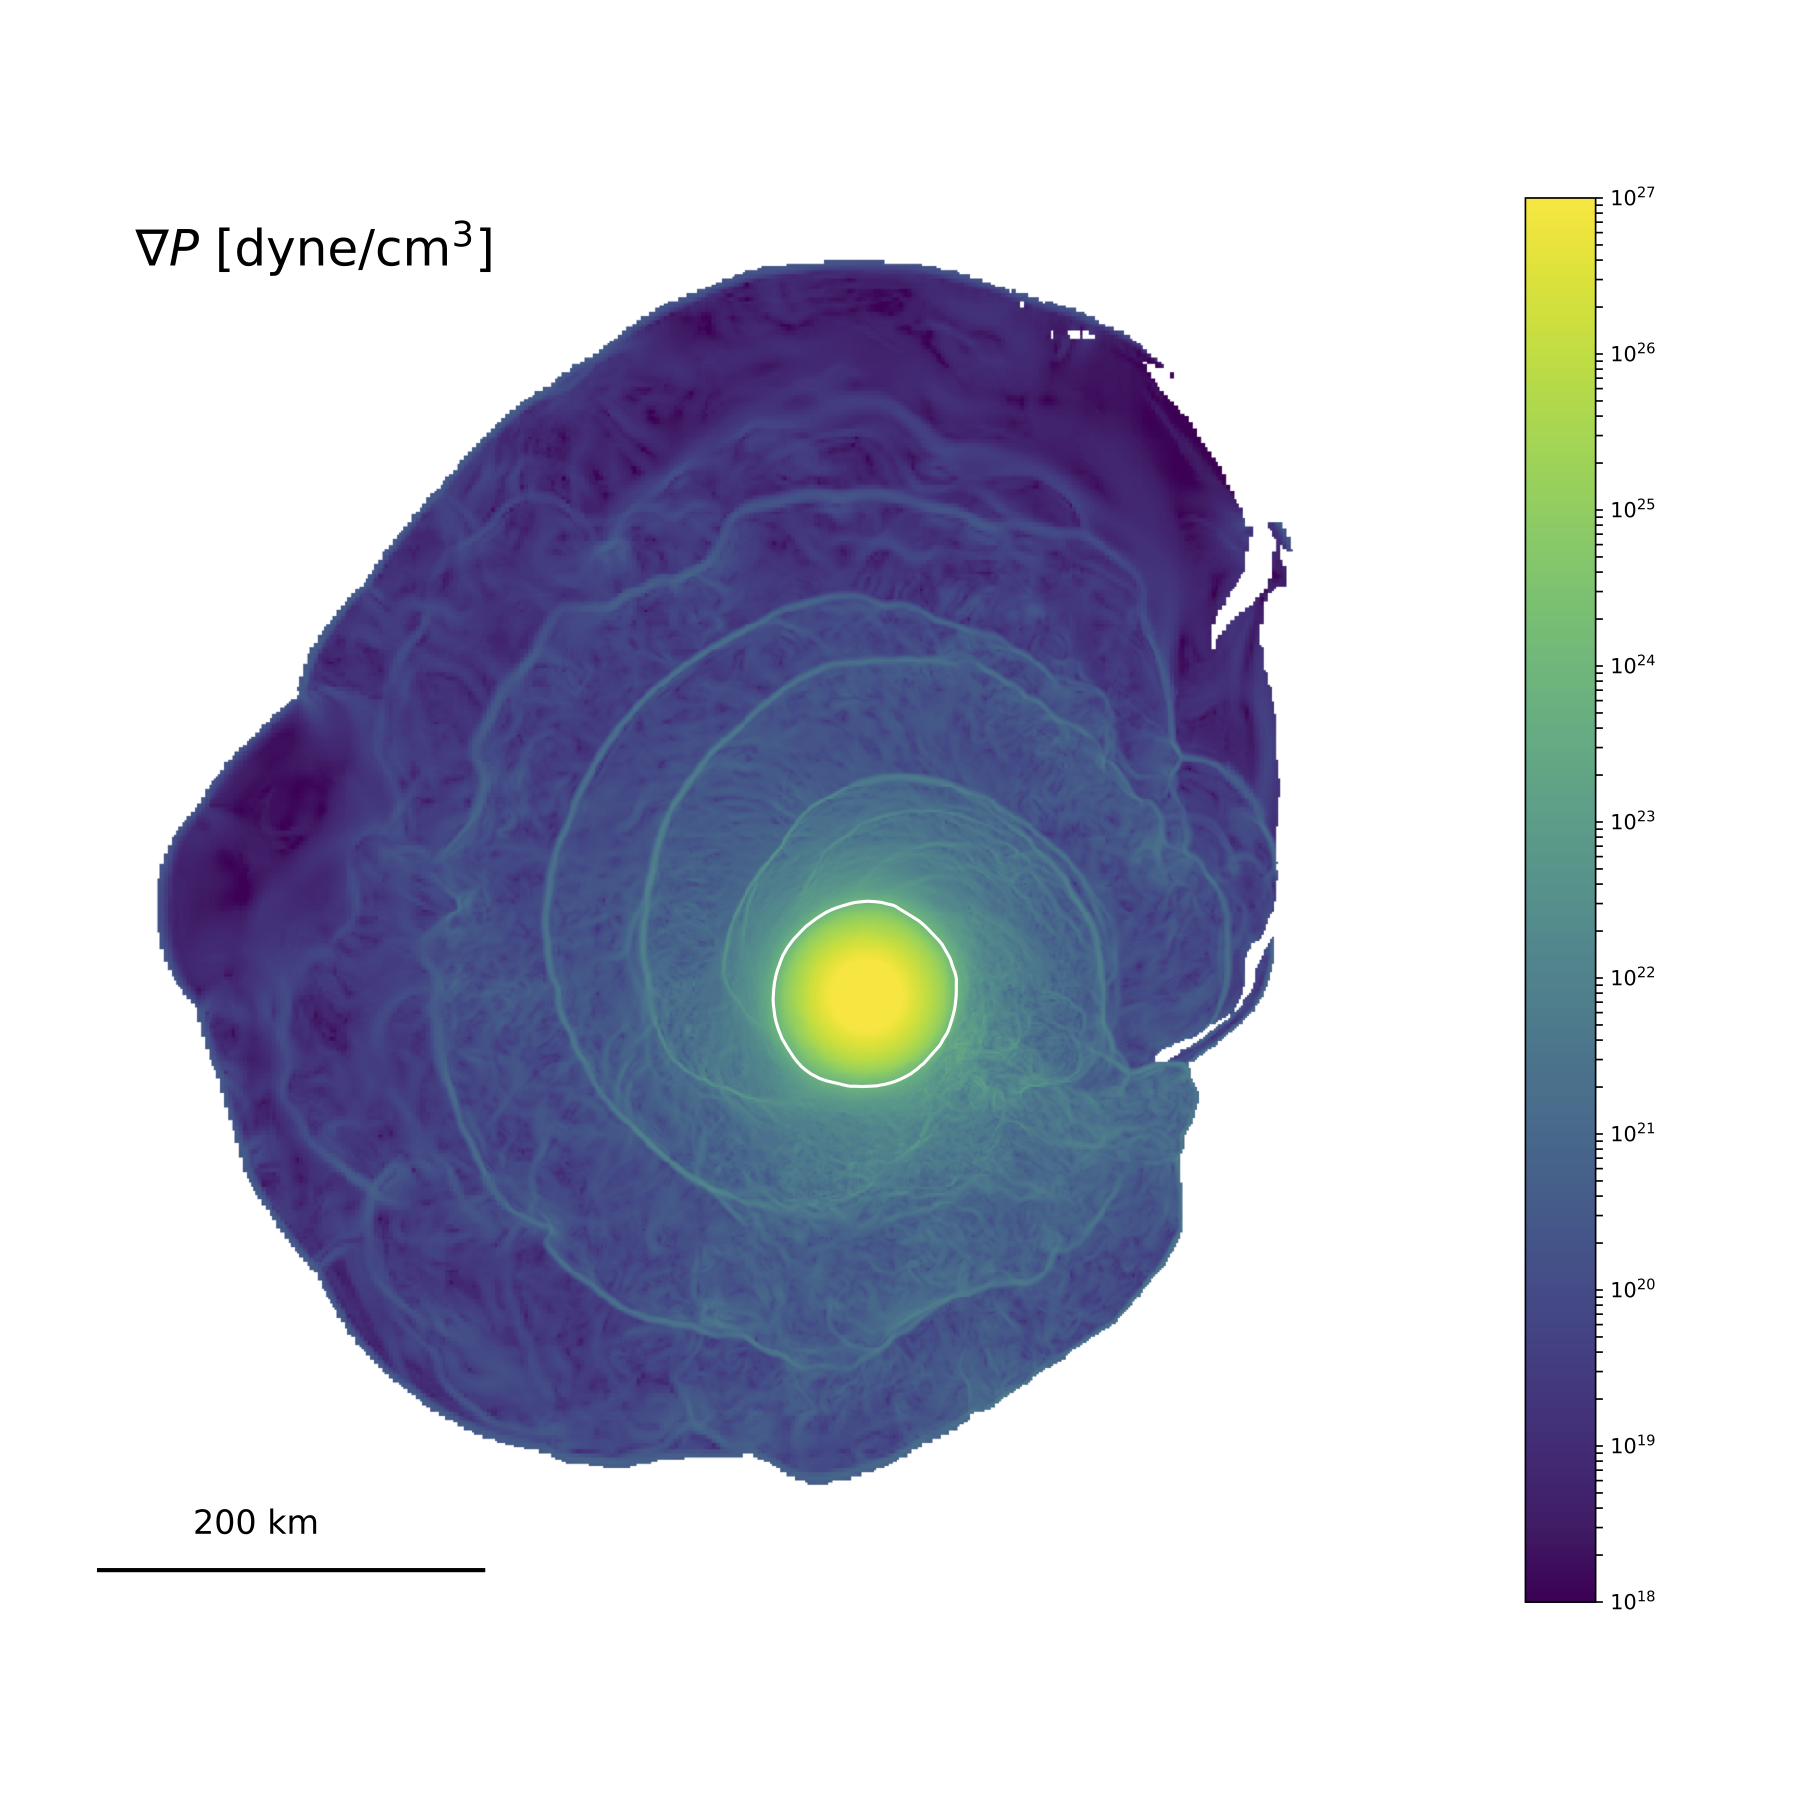
\includegraphics[width=2.9in]{./fig_gradp_m25_o110_b9_0566.png}
  \caption{Equatorial slice plot of the gradient of pressure from a 3D magnetorotational CCSN simulation run as part of our previous INCITE project. The development of a non-axisymmetric rotational instabity in the PNS leads to the generation of strong spiral pressures waves. The gravitational wave emission is also significantly amplified.}
  \label{f.gradp}
\end{wrapfigure}
This is, in fact, not very rapid rotation or field strength and so in these models we do not expect to see dramatic, magnetorotationally-dominated dynamics. 
Rather, we aim to explore the impact of plausibly typical rotation rates and field strengths on the CCSN mechanism. 

The 3D magnetorotational CCSN simulations are on-going and we fully expect to reach our target final simulation times by the end of Year 1. 
Already, we are seeing an impact of rotation and, to a lesser extent, magnetic fields.
We are already seeing that the rotating cases are closer to explosion.
The presence of magnetic fields is, so far, having little impact on the gross dynamics of the simulations, but for these initial field strengths it will take a longer period of evolution to build of substantial field strengths. 
The magnetic fields, even if weak, may still have an impact on the behavior of the turbulence in the gain region and the PNS.
This is an aspect of our simulations that we will analyze in detail once the simulations have reached later times. 
We will also look for the presence of a non-axisymmetric rotational instability in the PNS \citep{wheeler:2007, ott:2005}. 
In work based on simulations ran as part of our previous INCITE allocation, we have identified the emergence of such an instability for magnetic and rotating initial conditions. 
This instability can generate strong pressure waves that transport energy to the gain region, and also leads to very loud gravitational wave signals.
An image of the strong pressure waves is shown in Figure \ref{f.gradp}.

These simulations are currently running in the Capability queue on \mira. 
One simulation is running on \thet.

\subsection{3D Simulations of CCSN Progenitors}

One of the most remarkable and exciting results of recent 3D simulations of the CCSN mechanism is the discovery that  realistic non-spherical structure in the progenitor star can have a dramatic impact \citep{couch:2013b, couch:2015, couch:2015a, muller:2015, muller:2017, oconnor:2018b}.
The breaking of spherical symmetry is manifest in the turbulent convection driven by nuclear burning in the cores of massive stars.
As a massive star nears collapse, strongly convective burning in the Si and O shells surrounding the iron core can reach speeds of nearly 1000 km s$^{-1}$ and is characteristically very large in spatial scale \citep{Arnett:2011, couch:2015a, muller:2016a}.
These convective perturbations will reach the stalled shock shortly after core bounce and can aid neutrino-driven explosions by either enhancing the strength of post-shock turbulence \citep{couch:2015} or causing large scale ``forced shock deformations'' \citep{muller:2017}, or both.
These results serve to remind us that CCSN mechanism simulations are initial value problems and that the details of our initial conditions matter tremendously!
Our work inaugurated the era of detailed investigation into the impact of 3D progenitor structure on the CCSN mechanism \citep{couch:2013b, couch:2015a}.
As part of this INCITE project we are advancing the investigation into 3D progenitor structure substantially.
Specifically, we will simulate 3D progenitors including rotation and magnetic fields.

\begin{wrapfigure}[21]{r}{3in}
  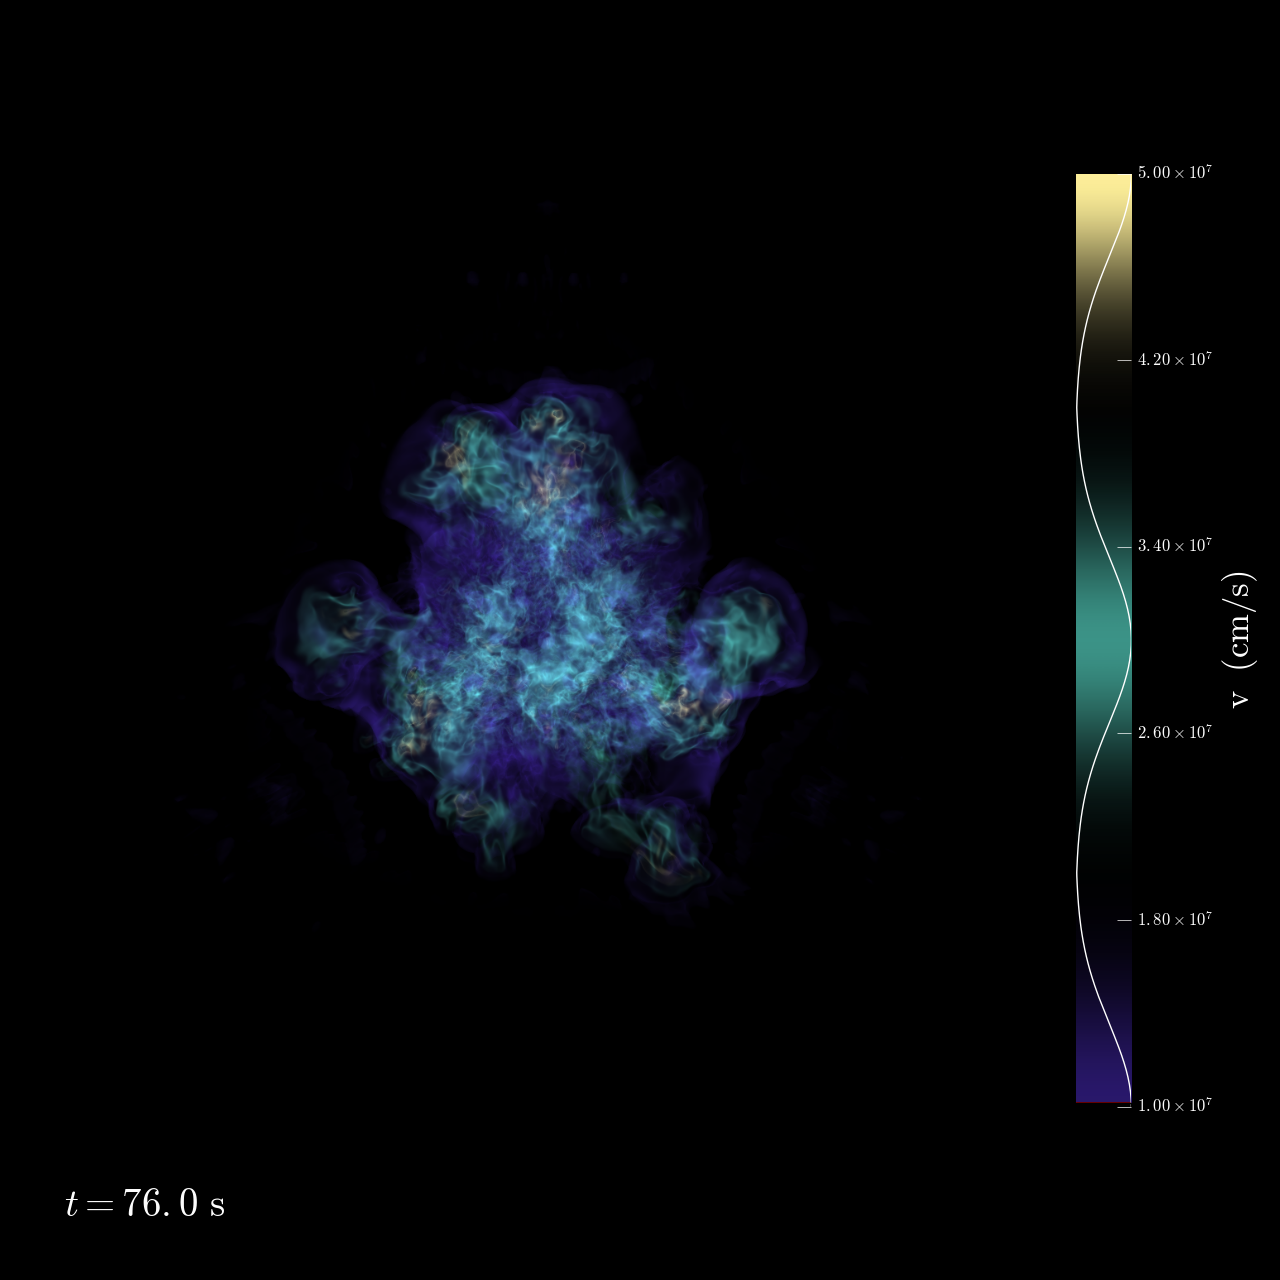
\includegraphics[width=2.9in]{./mag_vel_face_on_no_rot_prog3d_oct_vol_annotated_0076.png}
  \caption{3D progenitor simulation run in octant geometry as a forerunner of our planned Year 1 production simulations. Shown is the magnitude of the velocity. Peak convective speeds reach over 500 km/s prior to core collapse.}
  \label{f.progen}
\end{wrapfigure}
A key milestone for Year 1 is to carry out new, high-fidelity 3D simulations of the final minutes of stellar evolution to the point of iron core collapse.
For these simulations we will use the \spark MHD solver \citep{couch:2018} and include rotation and magnetic fields {\it for the first time ever} in a 3D CCSN progenitor simulation.
We are using 1D massive star evolution models constructed using MESA \citep{paxton:2011, paxton:2013, paxton:2015}, initialized in 3D approximately five minutes prior to core collapse.
We plan to run two, full-3D progenitor simulations in Year 1: one non-rotating, non-magnetic case and one rotating, magnetic case.
In the original proposal, we planned four 3D progenitor simulations in Year 1.
Our test simulations executed in octant geometry have shown that the expense of the simulations increases significantly as the stars approach collapse.
This is due to more vigorous nuclear burning in the core, increasing the expense of the nuclear network solve.
Therefore, in order to ensure that we can simulate sufficiently long time scales, we have opted to begin with just two simulations.


To this point in Year 1, we have made substantial gains in improving our simulation approach for 3D CCSN progenitors.
We have improved the OpenMP threading of our nuclear network code. 
We have improved the efficiency of the empirical load balancing approach our progenitor application uses. 
We have tested several approaches to the initial mapping of the 1D progenitor model to the 3D domain and have improved our approach to stabilizes the initial conditions. 
We have implement new, modern reaction rates for electron captures and for key carbon reactions.
And, importantly, we have run a test 3D progenitor simulation in octant geometry all the way to core instability and collapse.

We are now ready to begin our 3D progenitor production simulations on \mira. 
For the rotating, magnetic progenitor we are using a MESA model constructed using the magnetic field production and angular momentum transport model of \citet{spruit:2002}, as implemented for stellar evolution by \citet{heger:2005, paxton:2015}.
This model yields a realistic rotation profile and an estimate for the {\it strength} of the magnetic field as a function of radius in the star. 
There is very limited information about the 3D geometry of the field.
To address this, we are initializing the field in a random, divergenceless fashion with a typical strength matching the 1D MESA model estimate.
We will then allow the field to relax to a quasi-steady-state configuration.
This transition should occur on the rotational and convective time scale, both of which are about 30 s. 
We will simulate roughly 3 to 5 minutes of evolution up to core collapse.

\subsection{High-resolution Simulation of Magnetorotational Turbulence}

Our final simulation milestone for Year 1 is to execute a high-resolution simulation of magnetorotational turbulence in the CCSN gain region. 
For this simulation, we will use the ``rapidly'' rotating conditions described above.
We will restart the comparable fiducial resolution simulation at around 50 ms post-bounce and allow for higher resolution in the gain layer using AMR.
This simulation will require many more zones than the fiducial resolution case and we expect it to, in time, be a standalone Capability-scale simulation.
We are now ready to begin this simulation and will do so in the immediate future.

\subsection{Project Usage}

\begin{figure*}
  \begin{tabular}{cc}
    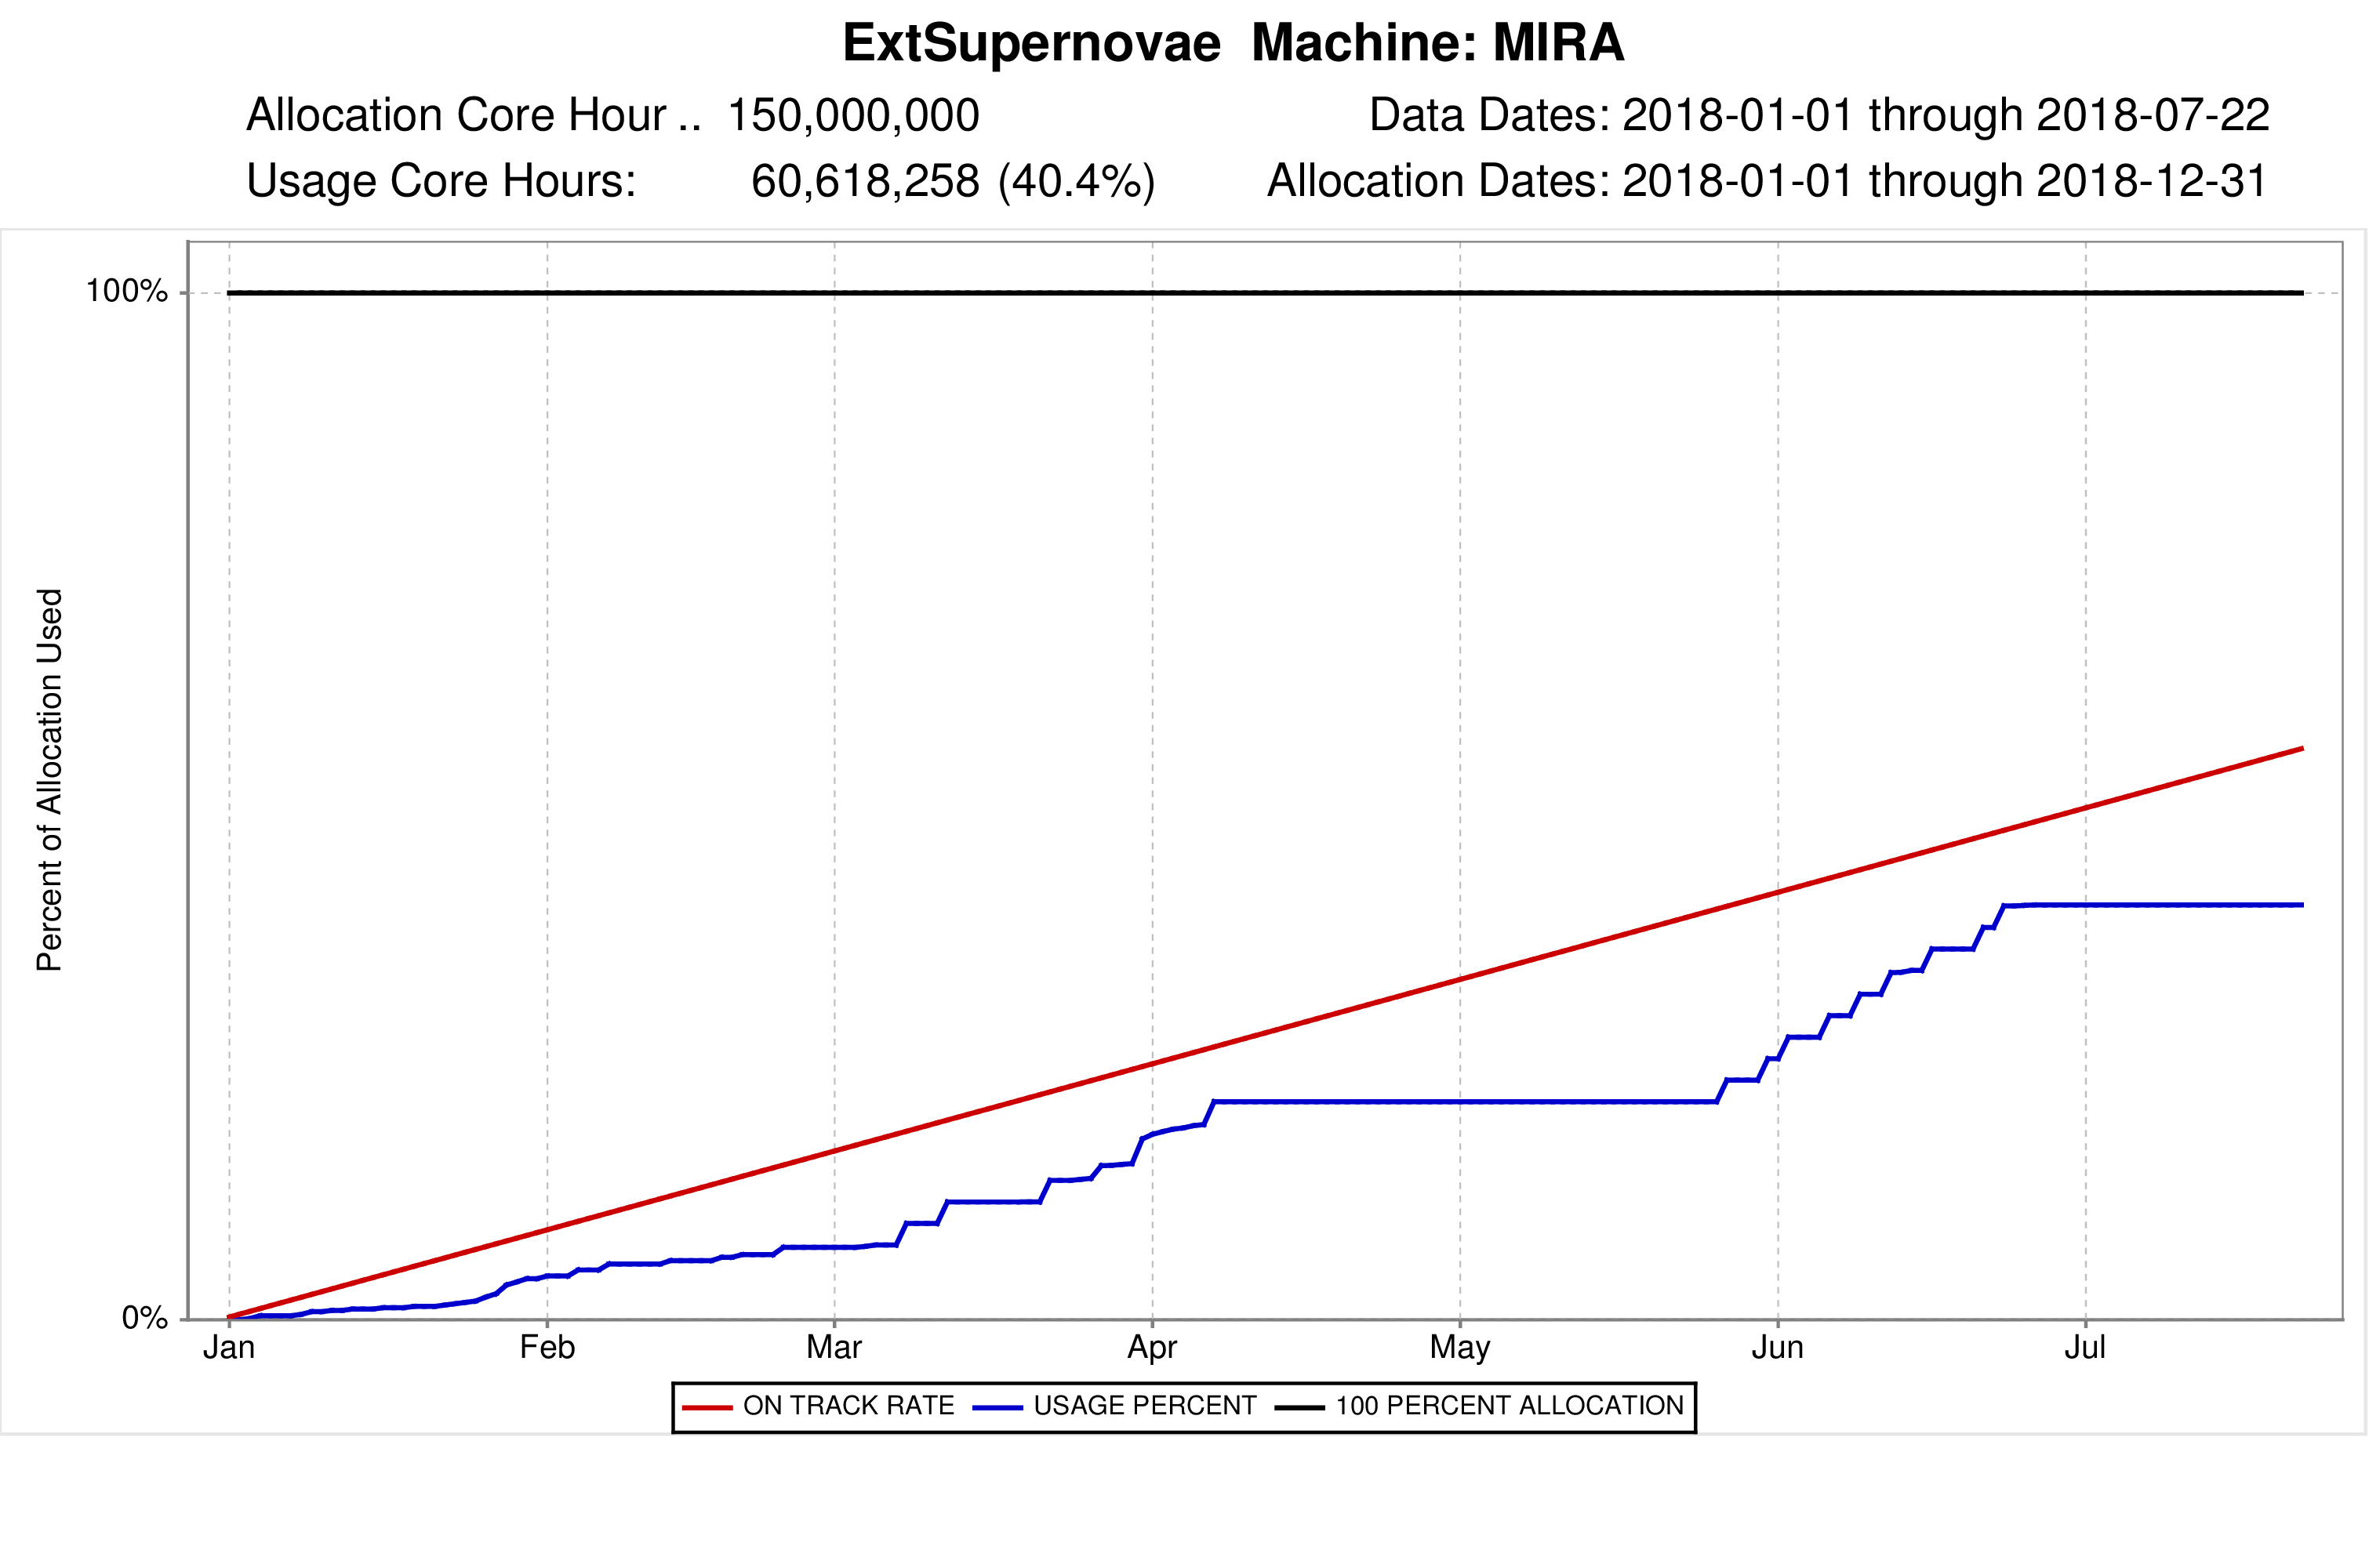
\includegraphics[width=3in]{./on_track_grapg-mira.png} &
    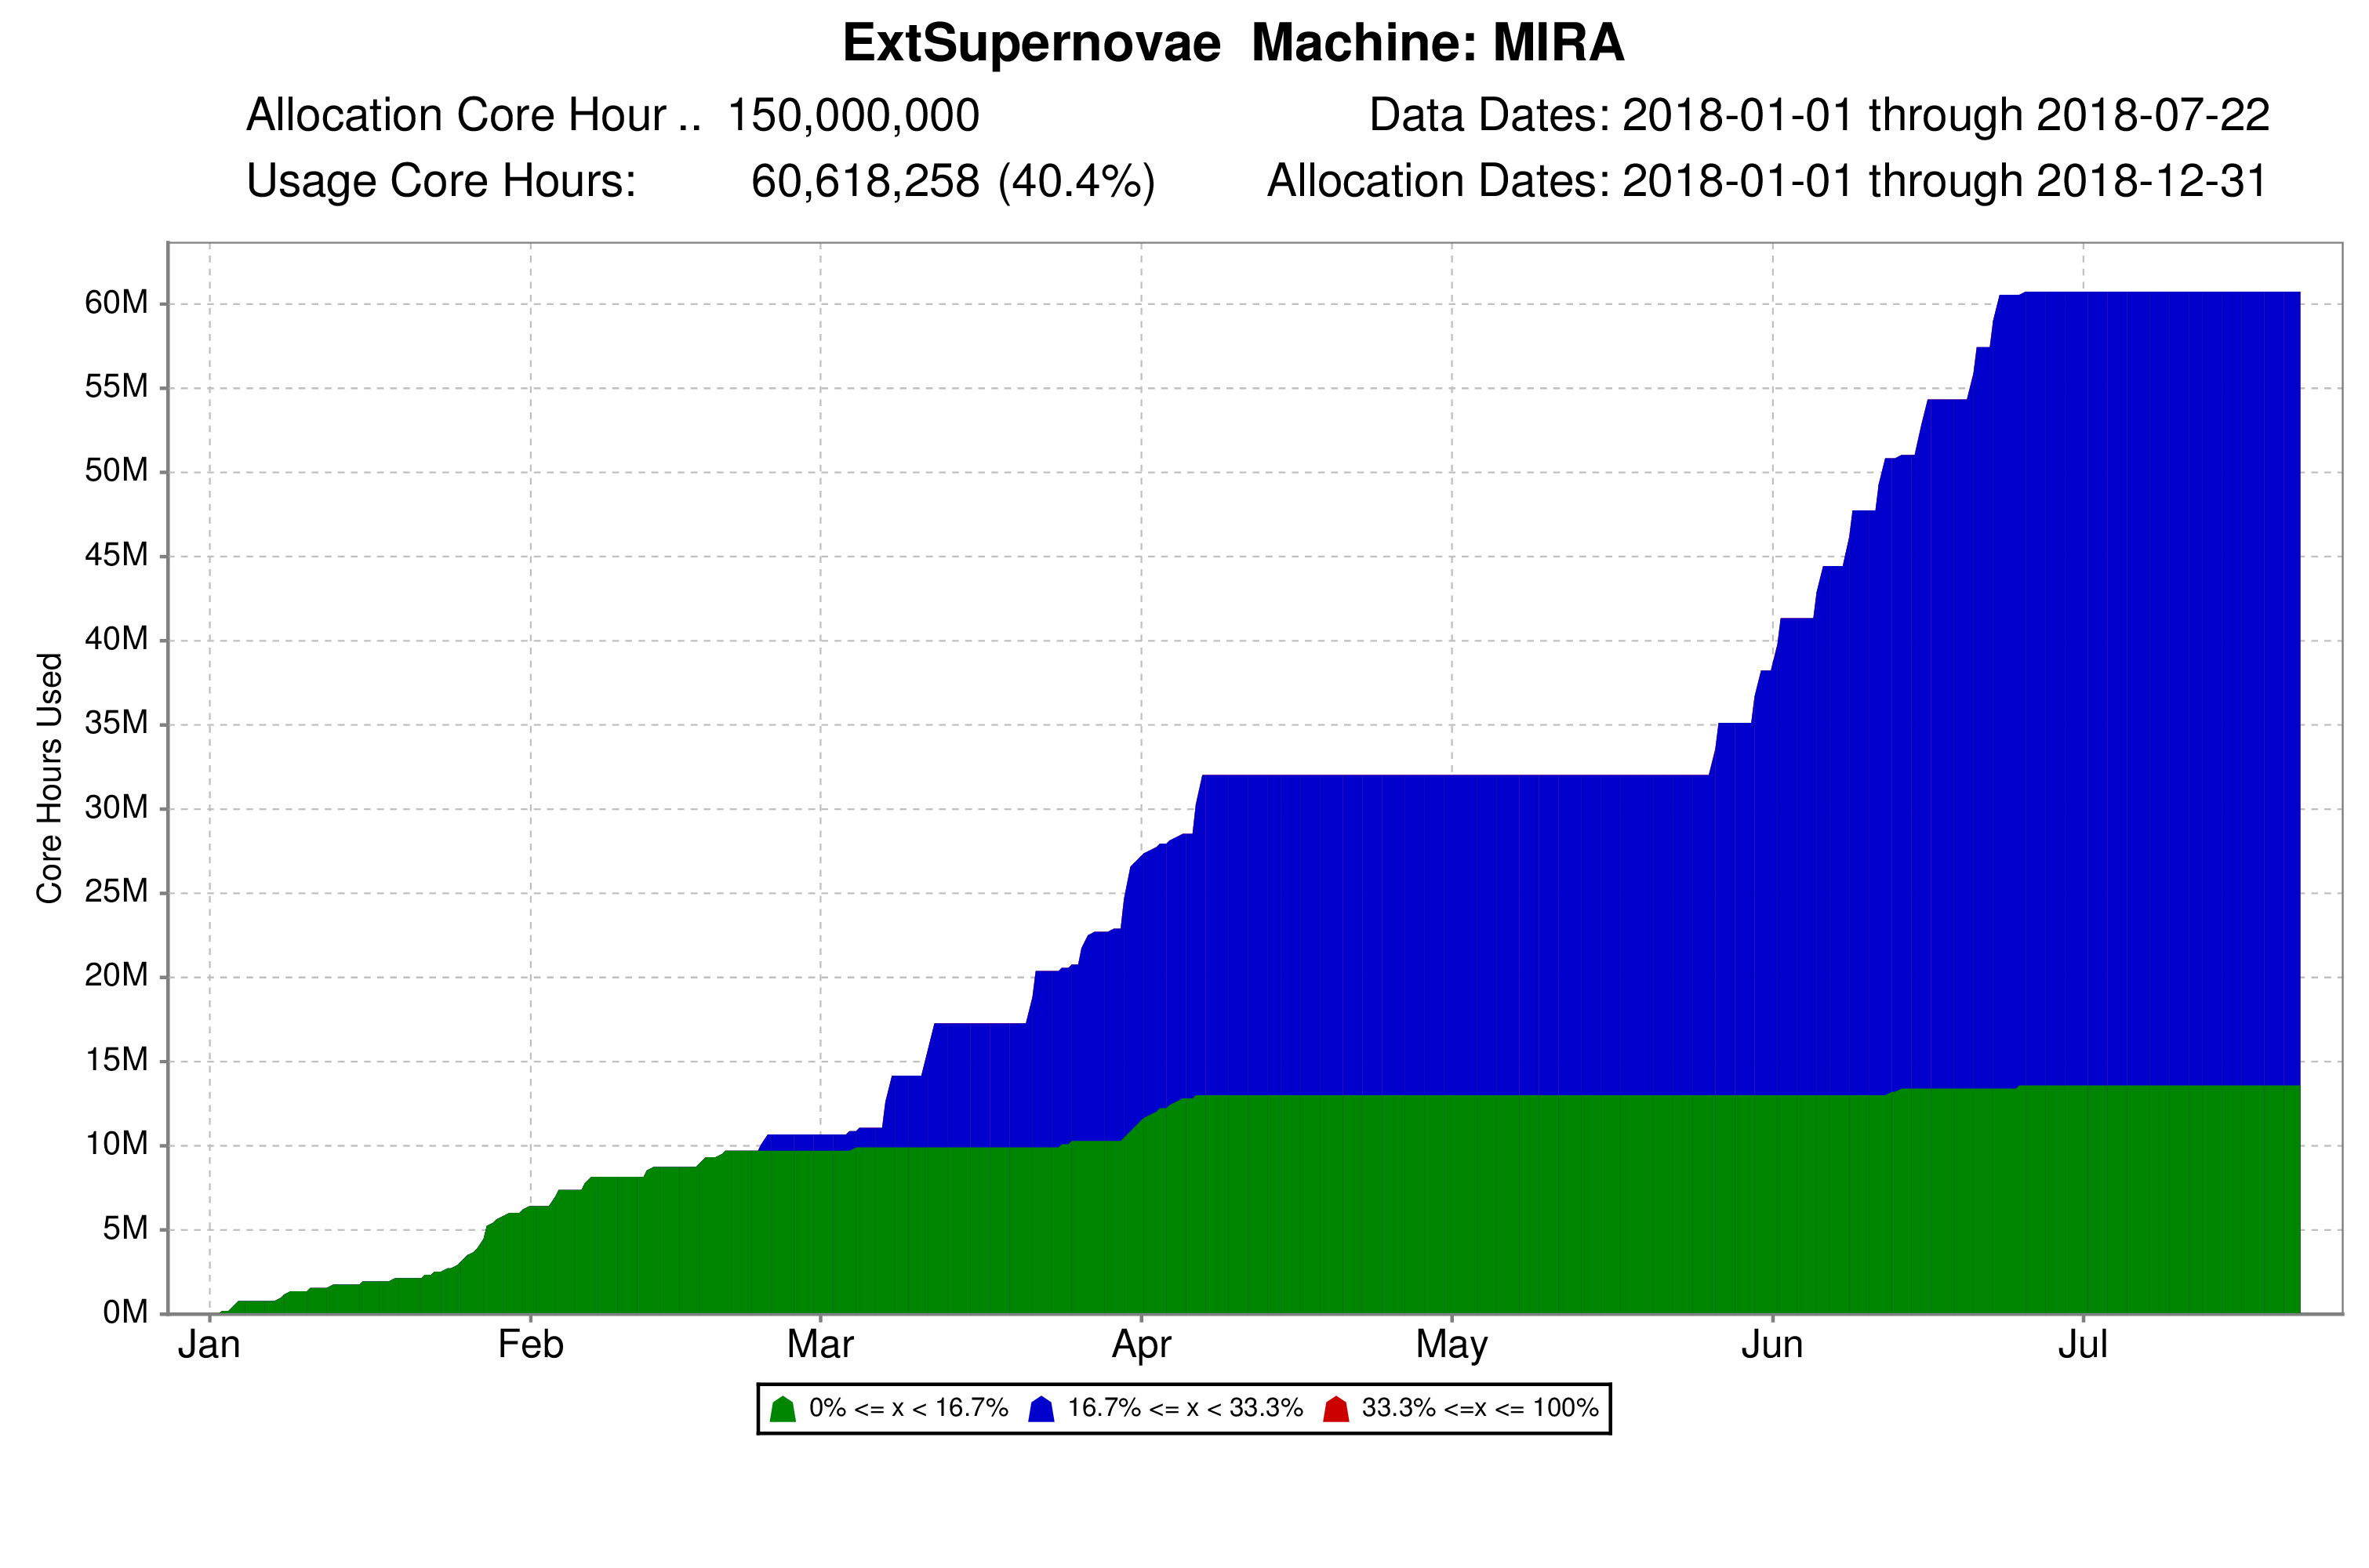
\includegraphics[width=3in]{./categorized_hours_graph-mira.png} \\
    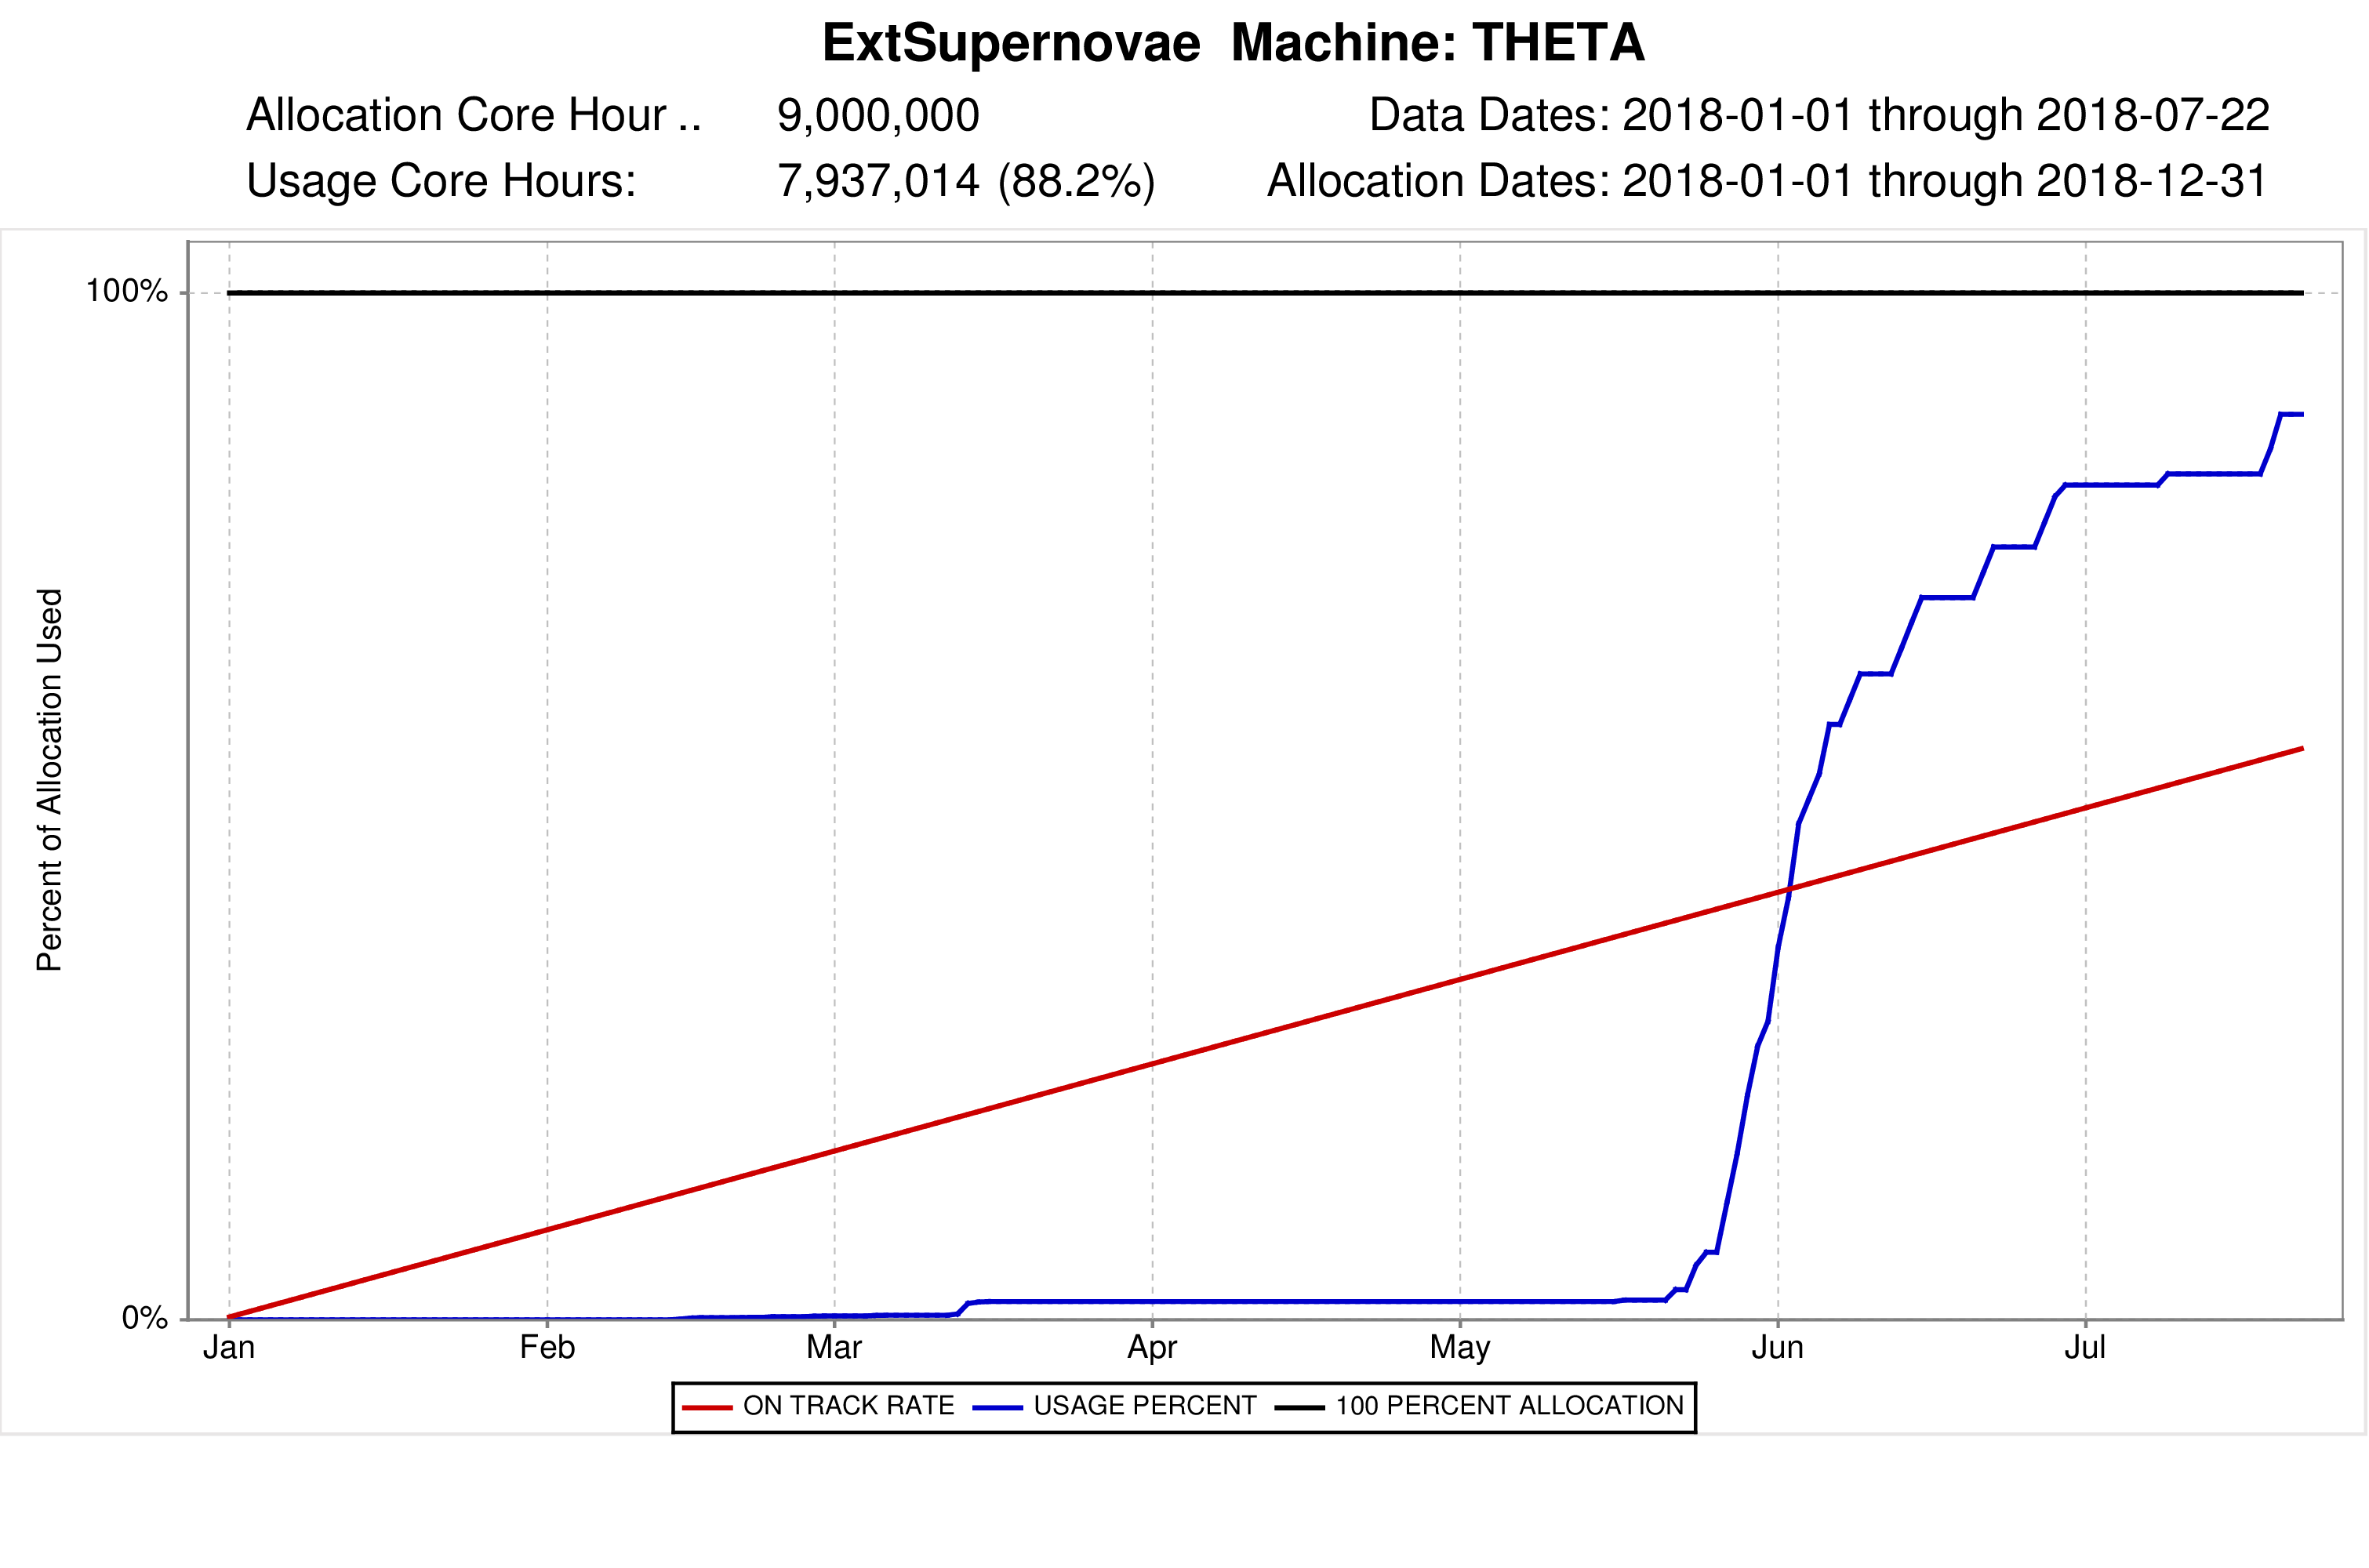
\includegraphics[width=3in]{./on_track_graph-theta.png} &
    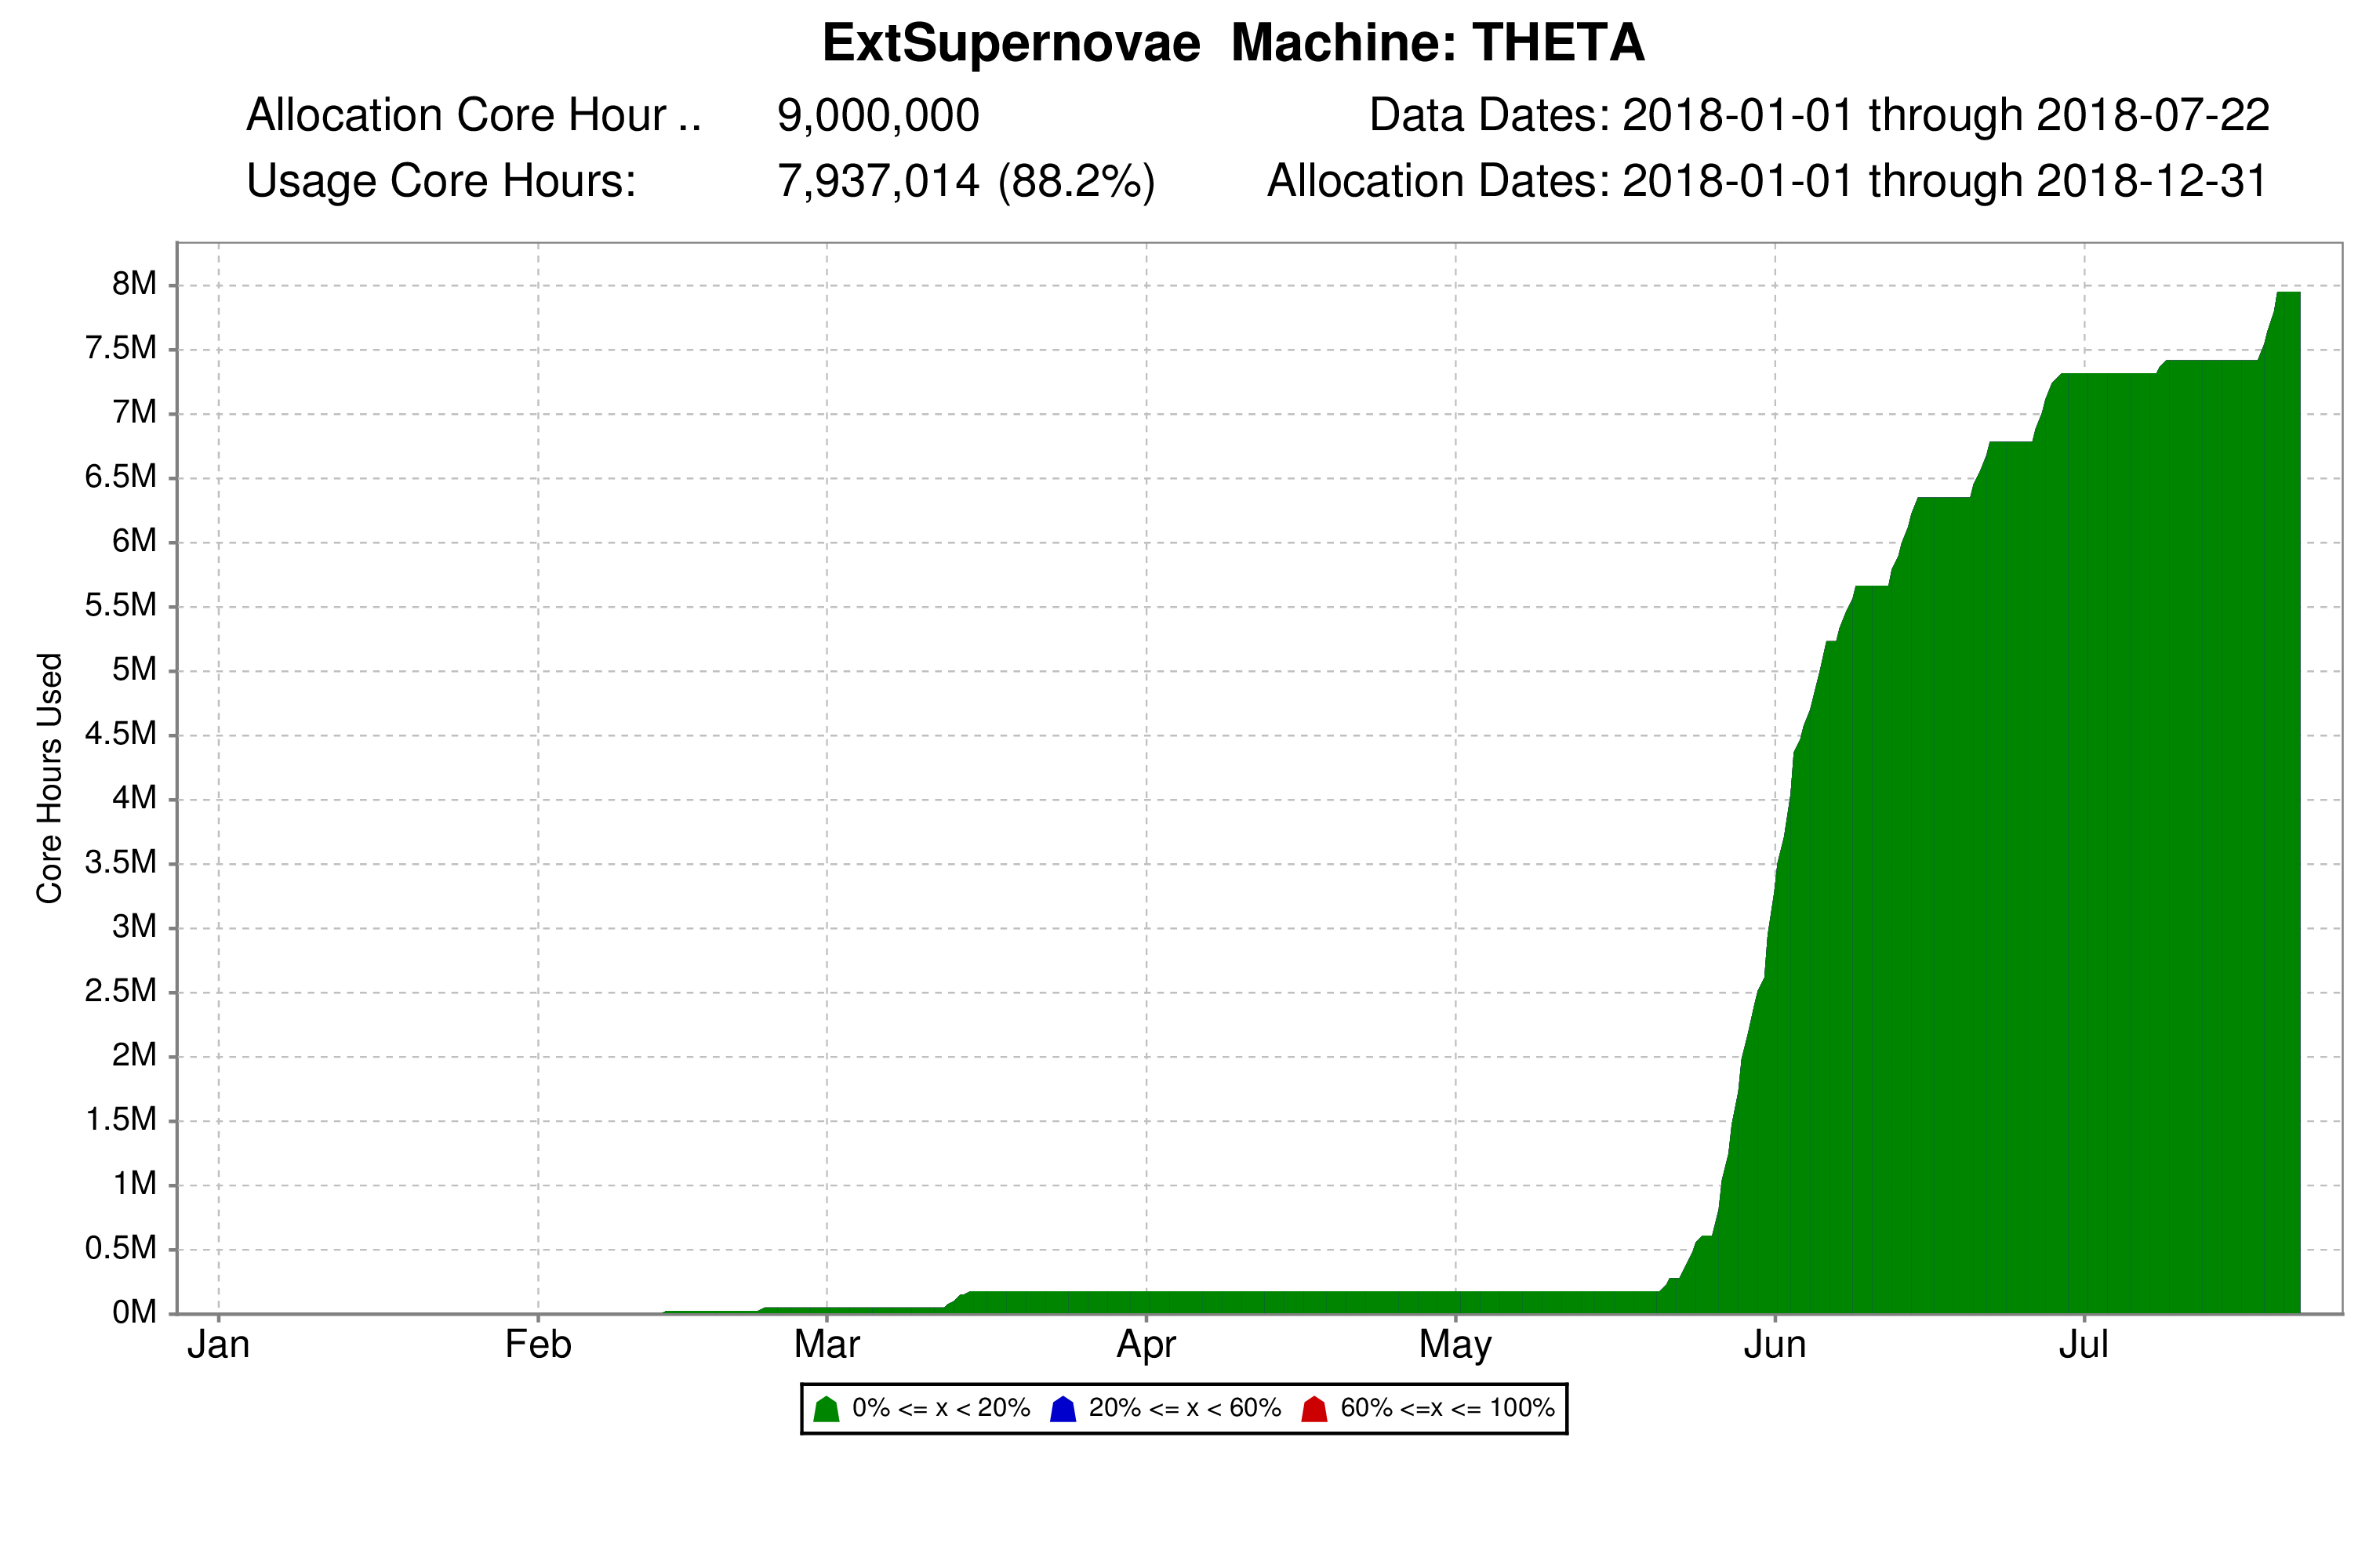
\includegraphics[width=3in]{./categorized_hours_graph-theta.png}    
  \end{tabular}  
  \caption{Usage of our allocation thus far in Year 1 for both \mira (top) and \thet (bottom).}
  \label{fig:usage}
\end{figure*}

Thus far, we have expended 60.6M core-hours on Mira, 40.4\% of our 2018 allocation (see Figure \ref{fig:usage}).
We are slightly behind the ideal usage curve, but in Q3 we will commence production 3D progenitor simulations and the high-resolution turbulence simulation, adding a two additional capability-scale jobs to our workflow.
Overall, we anticipate catching up quickly to the on-track usage curve.
The vast majority of our usage on Mira has been at the capability level.


We have so far expended 7.9M core-hours on Theta, 88.2\% of our 2018 allocation. 
At beginning of our allocation, we had technical issues with the Intel fortran compiler on Theta when enabling OpenMP.
After a few weeks of investigation, we decided to switch to GNU fortran compiler.    
After that, we moved one high-resolution production simulation from Mira to Theta 
and tuned our application on Theta to continue that simulation. 
A weak scaling test of restarting that simulation is shown in Figure~\ref{fig:theta}.
Figure~\ref{fig:theta} suggests that the performance is getting worse when using more than 300 nodes on Theta.
However, we noticed that after the maintenance on May 21, 2018, the wall-clock limit on Theta is limited to 6 hours 
with $> 256$ nodes and 9 hours with $> 384$ nodes.
Since our simulations require more than 50 of restarts, this limitation made it difficult to monitor our simulation.
Therefore, we have developed an automated job scheduling script to re-submit our job on Theta.    
    

\begin{figure}
  \begin{tabular}{cc} 
    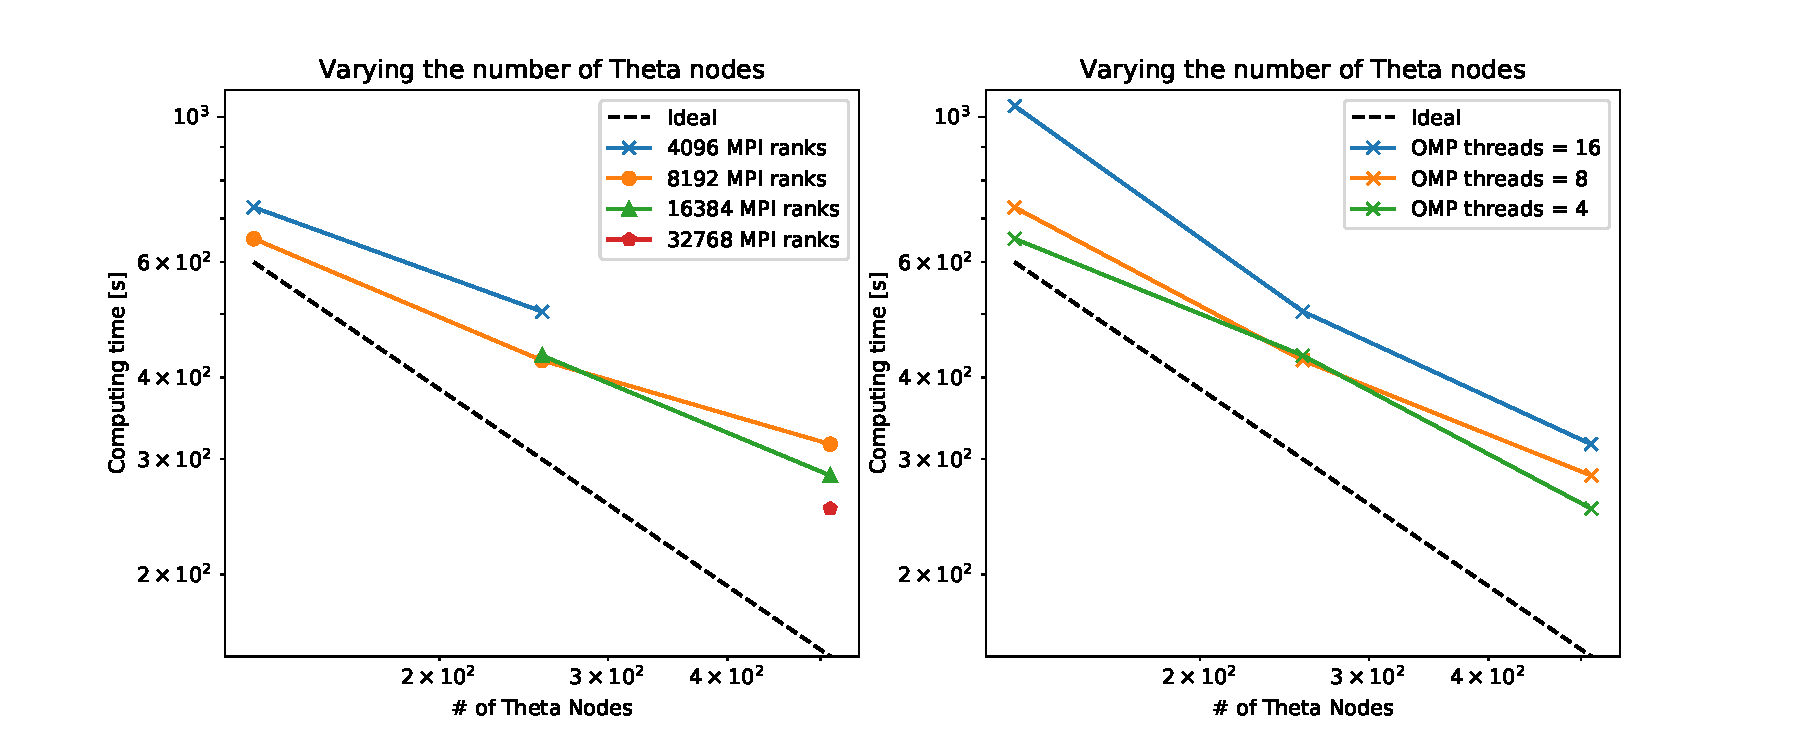
\includegraphics[width=6.5in]{fig_theta_scaling_j4.pdf}
  \end{tabular}
  \caption{Weak scaling test on Theta. Different colors represent different combinations of MPI and OpenMP tasks. }
  \label{fig:theta}
\end{figure}

\section{Code Development}

We planned two code development milestones for Year 1: implement a ``marching cubes'' approach for our EOS and opacity tables and develop a simulation workflow management tool in Python.
Both efforts are still underway.
While developing the marching cubes capability we found that we could significantly accelerate our table interpolations by reordering some of the large arrays.
This allowed for efficient vectorization by the compiler and sped up our table interpolations, both EOS and opacity, by about a factor of two. 
This improvement makes these aspects of our simulations relatively cheap, although the memory cost of the large tables is still high.
Nevertheless, we have downgraded the priority of implementing the marching cubes approach.\footnote{Never let optimization slow you down.}
We will still complete this implementation as person-power allows.

We have continued to develop workflow  tools for managing our large simulations on \mira and \thet. 
We have implemented new {\tt bash} scripts that automatically configure and submit restart jobs, which will substantially increase our queue throughput. 
We are incorporating these new tools into our existing Python tool chain.
We have also developed Python code to automatically configure and setup simulation parameter studies and generate job submission scripts. 
Work on this tool continues and we will implement functionality for some limited runtime visualization and automatic data archiving in the near future.

We have also made significant progress on other code development relevant to, but not directly planned as part of, this INCITE program. 
In our neutrino transport, we have implemented neutrino-electron inelastic scattering, an important process that we have so far only included during the 1D collapse phase of our simulations. 
We have also begun porting our \spark MHD solver to the DOE Exascale Computing Project (ECP)-supported AMReX framework. 
We are doing this within the new version of \flash that is being developed as part of the DOE ECP. 
We anticipate moving to the AMReX version of \flash in the future for our production simulations.

\begin{figure*}
  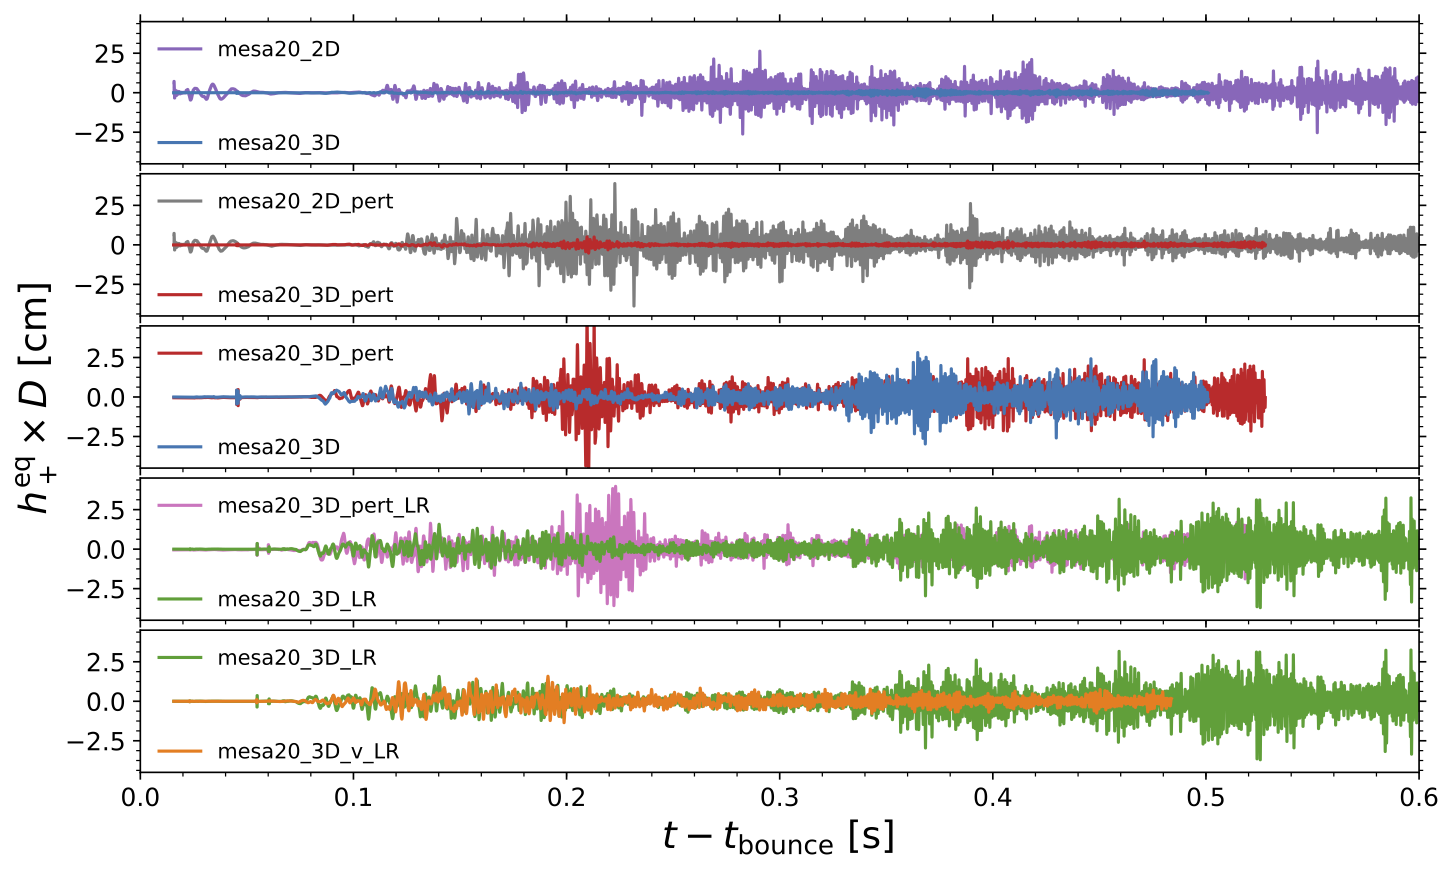
\includegraphics[width=6in]{./gw_trains.png}
  \caption{Gravitational wave strains from the 3D simulations of \citet{oconnor:2018}, carried out under a prior INCITE award. Our work showed for the first time that the presence of 3D structure in the progenitor star leaves a detectable imprint on the gravitational wave emission.}
  \label{f.strains}
\end{figure*}

\section{Fundamentally 3D Phenomena in CCSNe}

Recently, we submitted a publication detailing results based on simulations carried out under our previous INCITE award \citep{oconnor:2018b}.
This work includes several full 3D, high-resolution simulations using our M1 neutrino transport in \flash, representing over 100 Million core-hours of work on \mira.
In these simulations, we identify and analyze several essentially 3D aspects of CCSNe, including the presence of a new instability in the neutrino emission called the Lepton-number Emission Self-sustaining Asymmetry (LESA), first reported by \citep{tamborra:2014}. 
We are the first group to confirm the presence of the LESA in CCSNe and, since we use a very different transport approach, our work strongly implies this is not a numerical artifact but a real physical instability. 

In \citet{oconnor:2018}, we also show that the presence of the non-spherical, 3D progenitor structure has several important impacts on the CCSN mechanism. 
We show that convective motion in the progenitor can substantially increase the proximity to explosion.
We also showed that 3D structure in the progenitor can leave a measurable imprint on the gravitational wave emission from CCSNe that could be detected by, e.g., LIGO. 
The gravitational wave strains from our simulations are shown in Figure \ref{f.strains}.


% \begin{itemize}
%   \item 3D sims - running, starting hero 
%   \item improve 3D progenitors - init, c12ag, Langanke, threading
%   \item implement NES 
%   \item progress on workflow tool - only bash with simple python now
%   \item tuning for Theta 
%   \item have started working on EOS marching cubes...
%   \item port Spark to AMReX
%   \item 3D M1 paper
%   \item low-density EOS
% \end{itemize}




\renewcommand\bibsection{\section*{References}}
\setlength{\bibsep}{2pt}
%\begin{multicols}{2}
\bibliography{Achievements}
%\end{multicols}




\end{document}
